\frame{
\begin{block}{}
Numerical integration is a primary tool used by engineers and scientists to obtain approximate answers for definite integrals that cannot be solved analytically. 
\end{block}
}

\frame{
\frametitle{For example}
In the area of statistical thermodynamics, the Debye model\footnote{德拜模型} for calculating the heat capacity of a solid involves the following function; 
\begin{equation*}
\Phi(x) = \int_0^x \frac{t^3}{e^t-1} d t
\end{equation*}
\vspace{0.5cm}
Since there is no analytic expression for $\Phi(x)$, numerical integration must be used to obtain approximate values. 
}

\frame{
\begin{block}{}
the value $\Phi(5)$ is the area under the curve $y = f(t) = t^3 / (e^t - 1)$ for $0 \le t \le 5$ %(see Figure 5.1). 
The numerical approximation for $\Phi(5)$ is 
\begin{equation*}
\Phi(5) = \int_0^5 \frac{t^3}{e^t-1} d t \approx 4.8998922
\end{equation*}
Each additional value of $\Phi(x)$ must be determined by another numerical integration. 
\end{block}
\begin{columns}
\begin{column}{0.4\textwidth}
\begin{figure}
\begin{center}
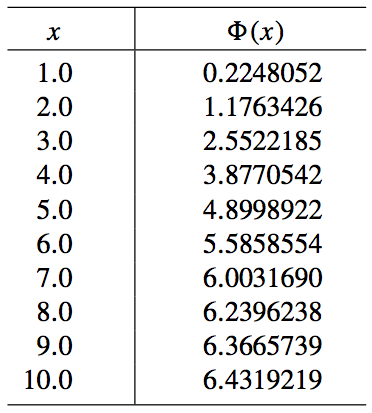
\includegraphics[width=30mm]{chap-5/tab_7-1.png}
\end{center}
\end{figure}
\end{column}
\begin{column}{0.6\textwidth}
\begin{figure}
\begin{center}
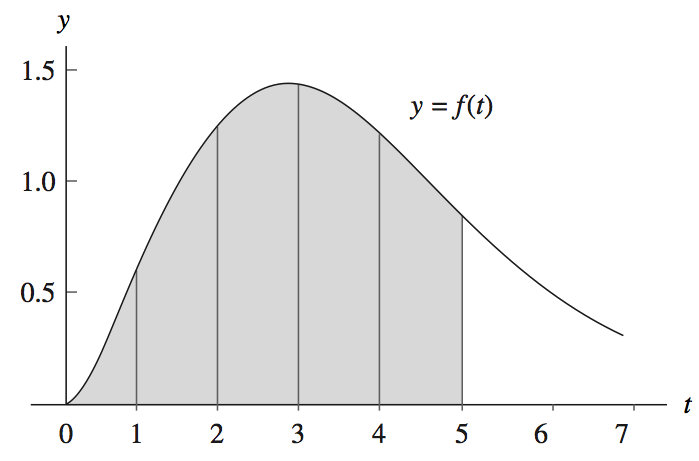
\includegraphics[width=50mm]{chap-5/fig_7-1.png}
\end{center}
\end{figure}
\end{column}
\end{columns}
}



\frame{
\begin{block}{}
\begin{center}
{\Huge The purpose of this chapter is to develop the basic principles of numerical integration.} \\
\end{center}
\end{block}
\vspace{3mm}
In the following Chapter , numerical integration formulas are used to derive the predictorcorrector methods for solving differential equations. 
}


